%----------------------------------------------------------------------------
\chapter{Áttekintés}
%----------------------------------------------------------------------------
%Mit csinál
%Mire jó (szerkesztés, finomítás?, import? új objektumok...)
%(technológia nélkül)


Kutatásom során megnéztem egy másik modellezőeszközt, ami a 'May' részlegesség feloldására nyújt megoldást és ezzel kapcsolatos döntéstámogatást szolgáltat\cite{Michalis}. A többi részlegesség kezelését nem teszi lehetővé. célom egy olyan modellező eszköz elkészítése, ami segítségével lehetséges részleges modelleket készíteni. Ehhez olyan vizuális szerkesztőfelület társul, ami megkönnyíti ezt a folyamatot. Ahhoz, hogy ez generikusan működjön egy általános modell szükséges. Így ez a modell tartalmazni fog objektumokat, attribútumokat és az ezek közti kapcsolatot kifejező referenciákat. Ezen felül minden elemhez lehetséges rendelni \textit{May}, \textit{Var} vagy \textit{Abs} részlegességet. Magához a modellhez pedig \textit{OW} részlegességet lehet rendelni.
\par
A kapcsolódó editor képes részleges modellt létrehozni és manipulálni. Lehetőséget ad új objektumok, attribútumok, referenciák létrehozására. Ezen elemekhez a már fent említett részlegességek rendelhetők. A szerkesztő a részlegességek feloldására, tehát finomításra is biztosít eszközöket.(áttekintő ábra lásd \autoref{overview})



\begin{figure}[!ht]
	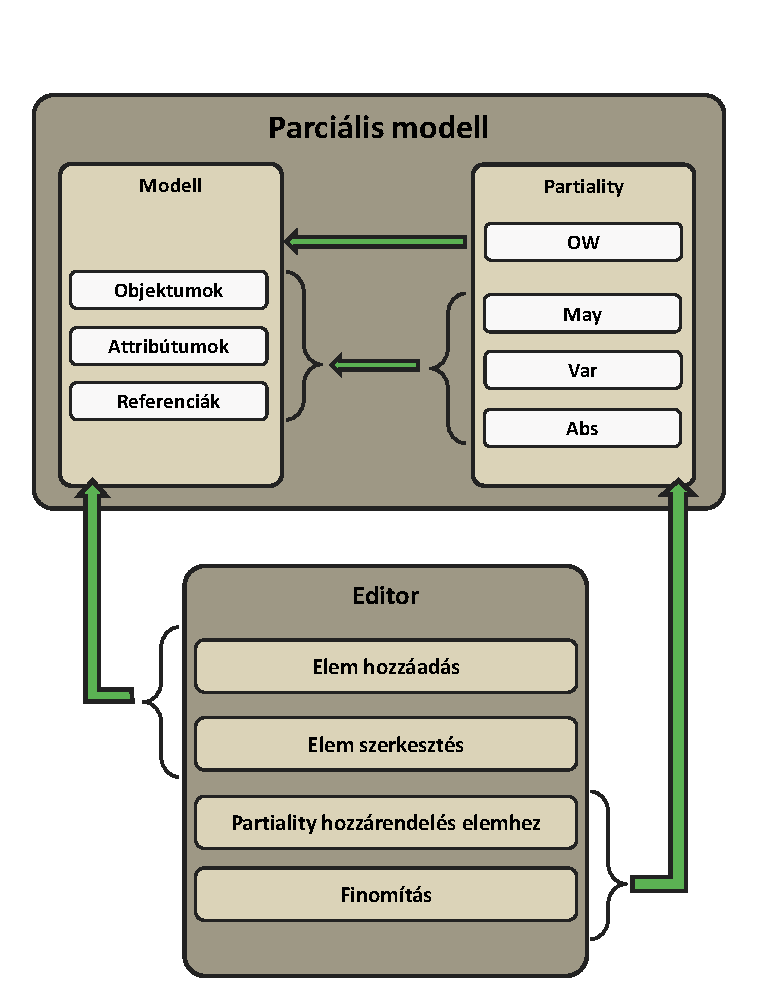
\includegraphics[width=150mm]{figures/overview.pdf}
	\caption{Részleges modell és a rajta végezhető műveletek} 
	\label{overview}
\end{figure}

